% REV00 Tue 20 Jul 2021 08:12:01 WIB
% START Tue 20 Jul 2021 08:12:01 WIB

\chapter{Sembilan}

% 11
\begin{figure}[htbp]
% h: here, where the figure appears in the text (use can always just use [h] )
% t: top,  top of the current page.
% b: bottom of the current page.
% p: page, top of the next available float space (sometimes end up being the end of the document).
\centerline{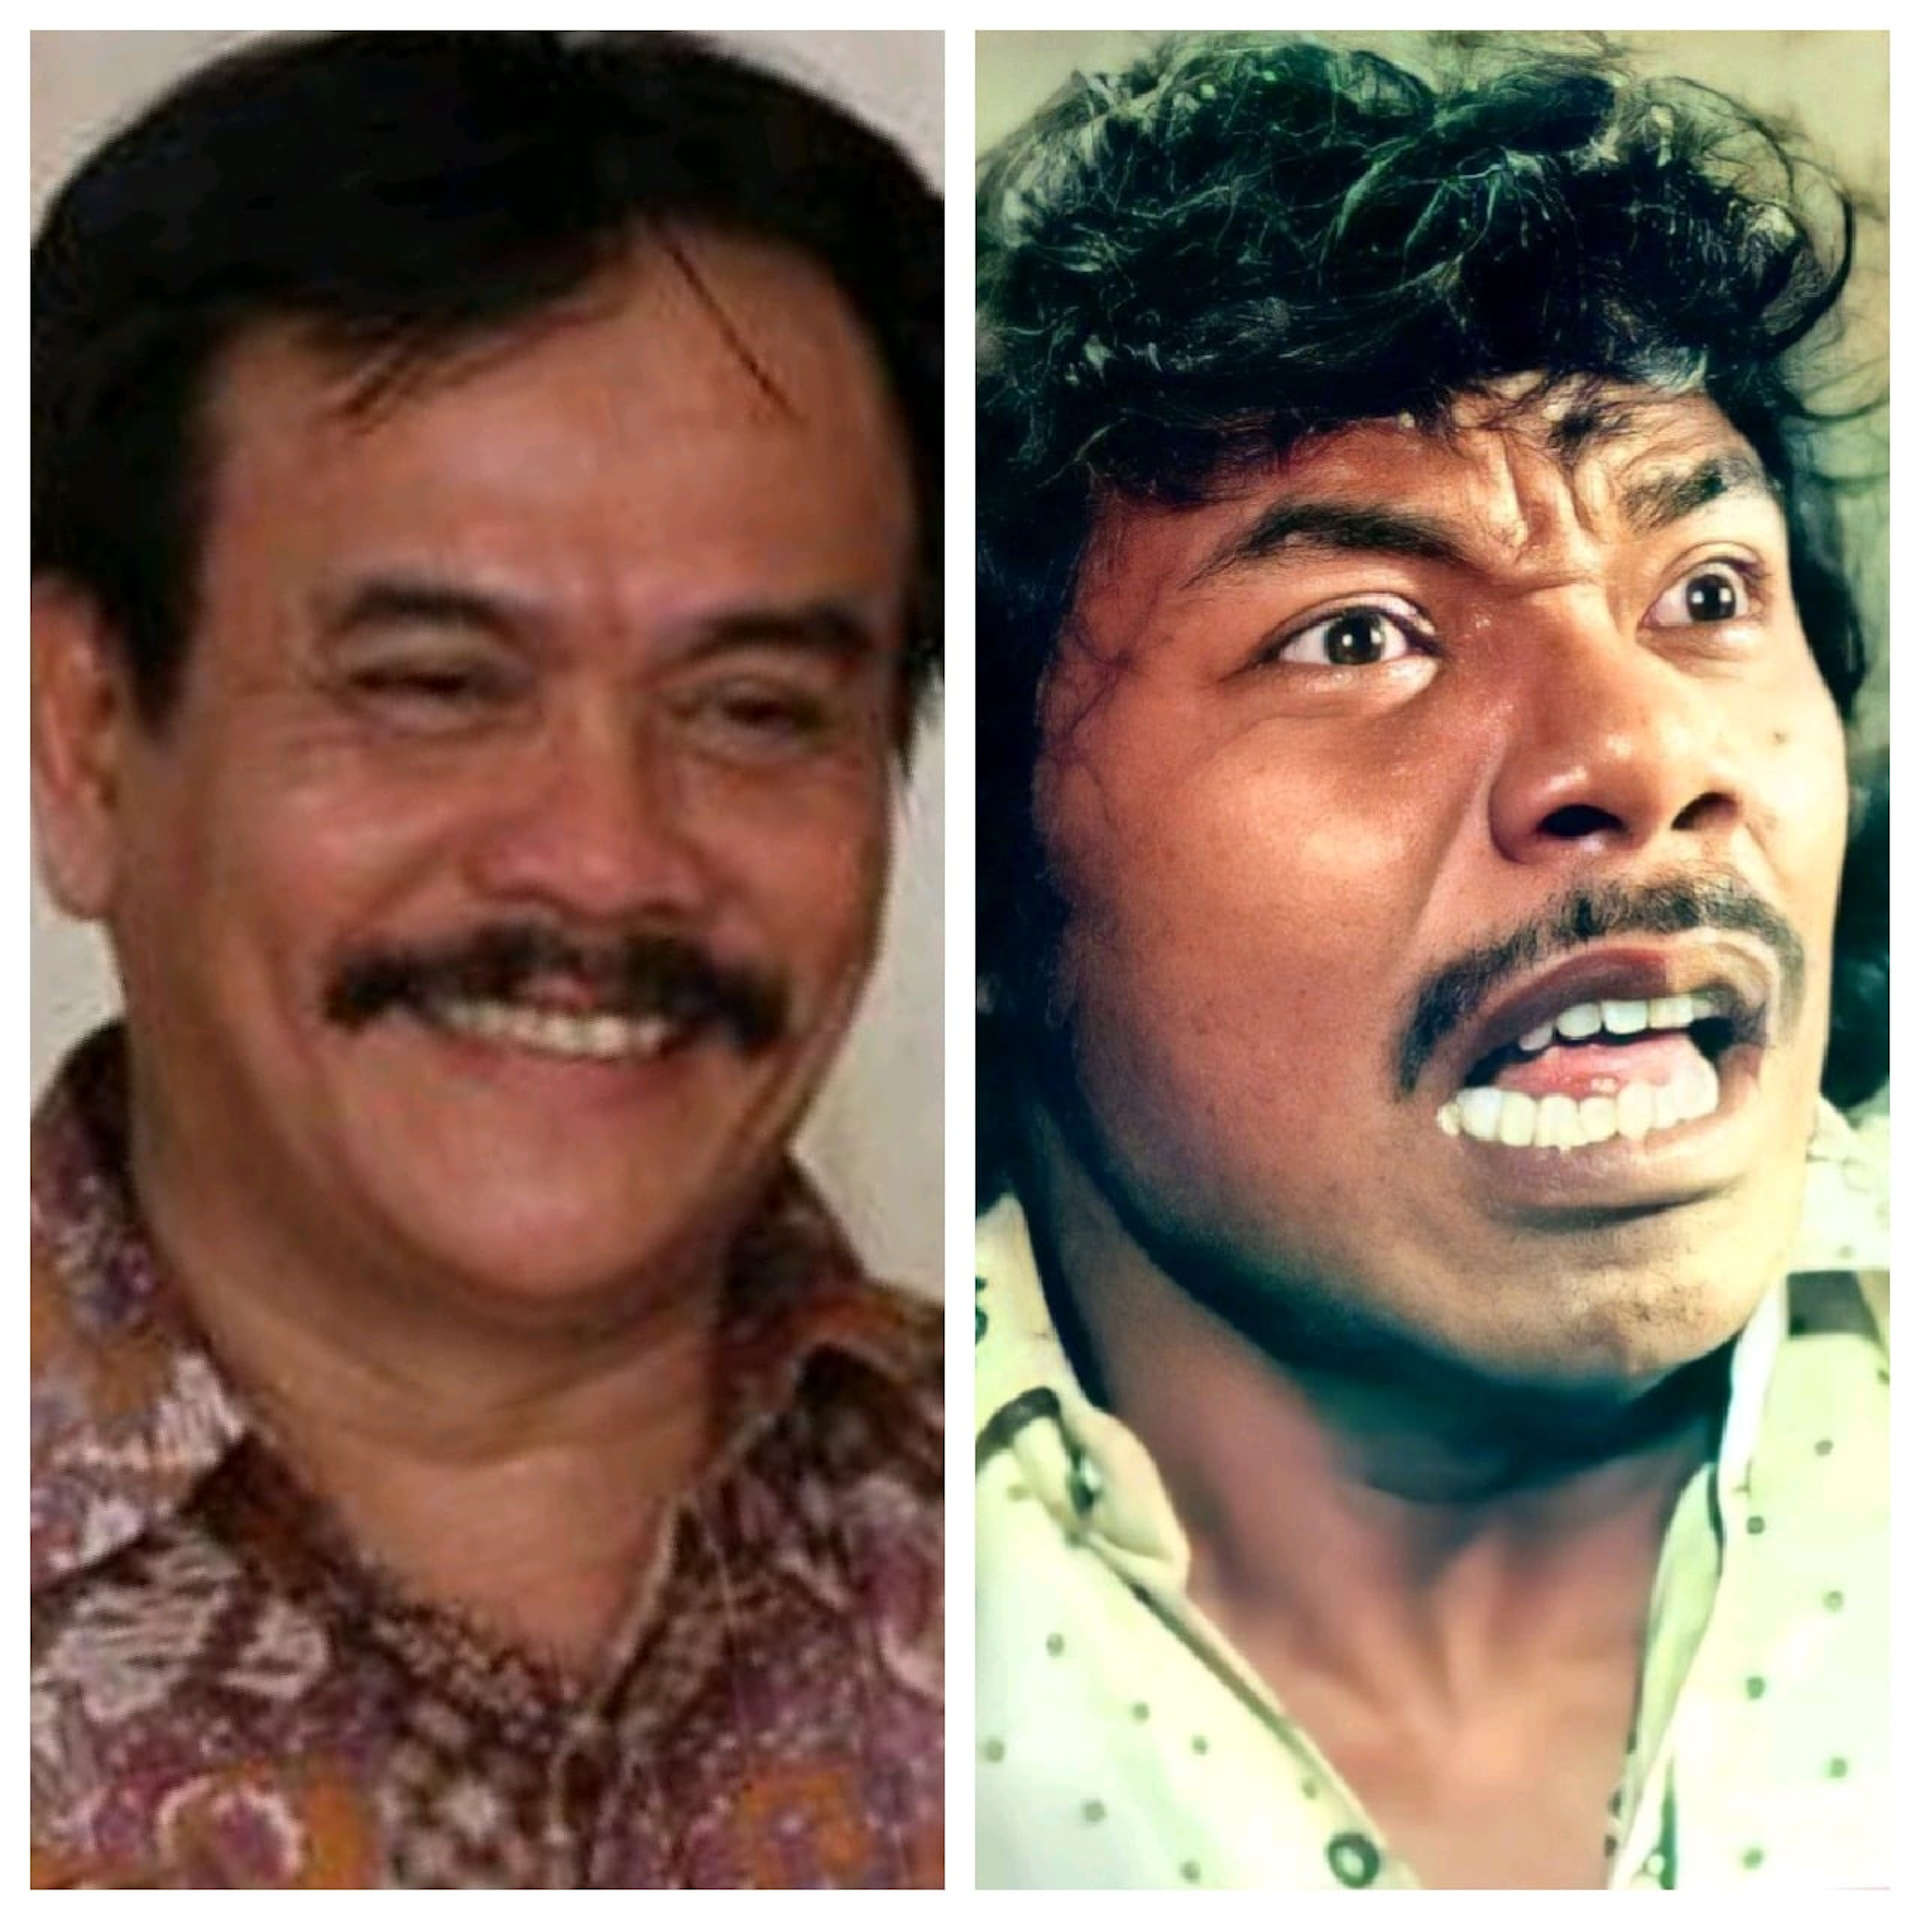
\includegraphics[scale=1.0]{01-09-01}}
\caption{“Bang Ben dan Satiri, dua pahlawanku dari Betawi”. Sumber: Internet.}
\label{01-09-01}
\end{figure}
%

Beranjak tahun ke-2, kami masuk ke Departemen yang kita pilih, dan terpilih untuk boleh memasukinya. Yang pertama kita hadapi untuk berkelahi adalah Himpunan Mahasiswa Fisika (Himafi), bukan Departemen Fisika. Ya, orientasi studi atau OS, atau lebih tepatnya perpeloncoan. Tempat kita digojlok.

Macam-macam lah perintahnya: Koran satu halaman (bukan satu lembar!), kue yang harus dibagi setengah secara berantai (bayangin dulu…), scott-jump, suntik bumi, dan semua kegilaan lain buat kita semua yang bukan ‘seksi mampus’.

Nah, itulah Satiri, dia pura-pura mampus, digotong seksi mampus ke RS Borromeus. Kadal mau dikadalin. Hahahah…

Semua aturan perpeloncoan di dunia itu sama:

\begin{enumerate}
\item Junior selalu salah;
\item Kalau Senior salah, lihat aturan nomor satu; dan,
\item "Ya, dewa…" itulah jawaban pertama dan satu-satunya jawaban yang harus kita berikan.
\end{enumerate}

Setelah dua minggu babak belur dipelonco setiap hari dari jam 6 pagi hingga jam 11 malam, kita dibawa camping. Kalau tidak ke hutan pinus Cikole, Utara Bandung, bisa juga ke Ranca Upas menuju Situ Patengan (kita sering melafalkannya sebagai Patenggang), Selatan Bandung. Mana saja asal hutannya lebat, banyak genderuwonya, dan dinginnya alang kepalang.

Tibalah kita pada puncak acara: JURIT MALAM. Pas tengah malam kita disuruh menelusuri jalur hutan belantara yang ditentukan Panitia, dengan hanya berbekal satu lampu senter saja. Kita dilepas berdua-berdua dengan jarak 10 menit. Biasanya ada lima pos yang harus kita lalui, dan di setiap pos itu ada tugas dari senior yang intinya kita dikerjailah di sana.

Seingatku Satiri dipasangkan dengan teh Lilis. (Teh Lilis adalah bidadari yang paling dihormati dari enam “Physics’80 Angels”). Lepas dari Pos-2, muncul ide gilanya.

“Teh Lilis, kita berhenti di sini dulu. Teteh diam saja di situ ya...”

“Emang Satiri mau apa?” katanya dengan nada Sunda yang empuk dan lemas.

Belum selesai teh Lilis bertanya lebih jauh, Satiri berteriak ke arah belakang:

“Wooi, jongkooook… Jalan jongkok ke sini!” hardiknya. Siapa yang dihardik? Pasangan tim yang ada di belakangnya!

“Ya, dewa…” begitulah mereka melata sambil jongkok mendekat. Tak lupa dengan kedua tangan yang dirapatkan di belakang kepala. Otomatis, walau tanpa diminta.

Dasar gelo. Lima pasangan teman-temannya sendiri kena dikerjai, termasuk Boy:

“Angkat muka. Lu enggak tau gua siapa?!” bentaknya.

“Wasssah… dasar Bangsaat!” Boy hanya bisa mangkel, sontak berdiri memendang Satiri dengan canda, dan mereka tertawa bersama.

Oia, “Bangsat” atau “Bang Sat” itu adalah panggilan tersayang buat Satiri. Bang Tiri itu cuma panggilan akrab, hormat, atau digunakan sebagai orang ketiga.

Di hari terakhir masa OS seperti itu tentunya mental semua orang sudah down, dan ngantuk. Disuruh apa saja pasti mau, asal acara cepat selesai. Hanya Satiri yang tahu itu…

Bertahun-tahun kemudaian tidak pernah kudengar ide gila seperti itu. Sama juga dengan kegilaannya menggunakan kuitansi tukang sayur dan cap himpunan.

Hidup itu bukan hanya Fisika. Hidup itu ya harus dihidupkan!

Tahun berikutnya, ketika kami mendapat giliran mengelola OS, Bejo jadi Ketua, Satiri jadi seksi kesenian. Seni suka-suka. Ada yang dikasih nama: Nyongclo, Goceng, Kantil, dan apapun nama yang ia bikin sekenanya.

Oia, nama ini secara tradisional harus ditulis tebal pada karton segede gajah, dilaminating, dan digantung di dada kita. Nama itulah yang jadi nama resmi selama OS.

Gantungan nama akan dibakar pada acara api unggun perdamaian setelah selesai jurit malam. Menandakan akhir masa OS dan semua senior resmi menjadi saudara, teteh dan akang.

Di saat itulah Satiri dengan senang hati menyenandungkan kocokan gitar dangdut untuk salah satu balada kesukaannya:

\begin{verbatim}
... engkau kejam engkau sadis kekasihku,
yang egoistis tapi manis,
seperti pala manis

kau putuskan tali cintaku,
yang tebal seperti tambang kapal

hatiku kini hancur luruh,
bagaikan cermin yang jatuh dari helikopter
tak mungkin bersemi lagi..

Reff.:
kini tiada lagi cinta,
yang tinggal cuma celana kolor

hidup trasa hampa udara napasku,
sesak seperti menghirup asap tabunan

kan kubawa luka hatiku,
berlari marathon lewat jagorawi

smoga aku dapat melupakan,
wajahmu yang bulat,
seperti bangkuang bogor

ohoooooo kekasih
ohooooooi...

(Benyamin Sueb, "Cintaku Berat Diongkos"
\end{verbatim}

\vspace{10mm}

Sumber tulisan asli \url{https://www.facebook.com/reno.alamsyah.94/posts/10226555102769891}

